\chapter{Ferromagnetism and the Ising Model}

In this Chapter  a brief introduction to ferromagnetism is presented, from the history and significance of the Ising model, to the joint density of states and relevant thermodynamic relations and properties obtained from it.

\section{Ferromagnetism}

Magnetic materials are critical in our modern society, since they have very broad applications in our daily lives. For example, there are magnetic materials in every speaker and microphone, hard-drive disks on our computers, they play a big role in medicine where they are used in body scanners (usually in MRI machines) and together with applications in electric motors, transformers and generators \cite{Gutfleisch2011}. Magnetic materials can be classified in terms of their magnetic properties, such as diamagnetism, paramagnetism, ferromagnetism, and so forth \cite{Griffiths}. 

\begin{figure}[ht]
\centering
\subfigure[]{%
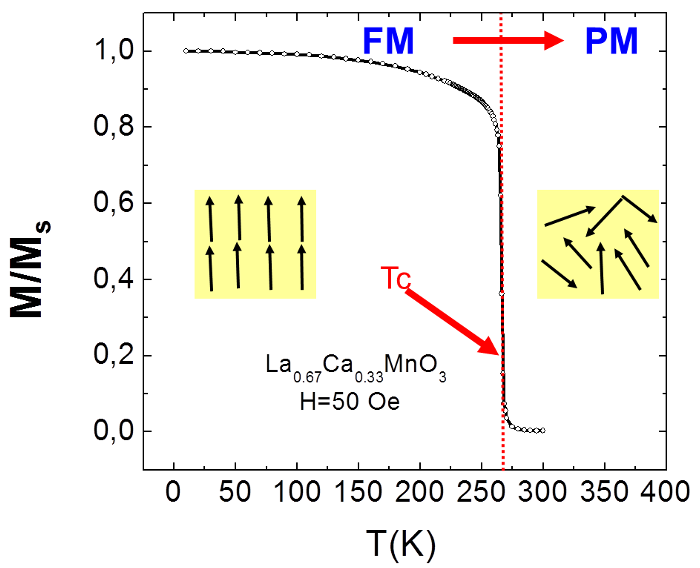
\includegraphics[scale=0.4]{phase_transition.png}
\label{tese_JA_fig1}}
\quad
\quad
\quad
\subfigure[]{%
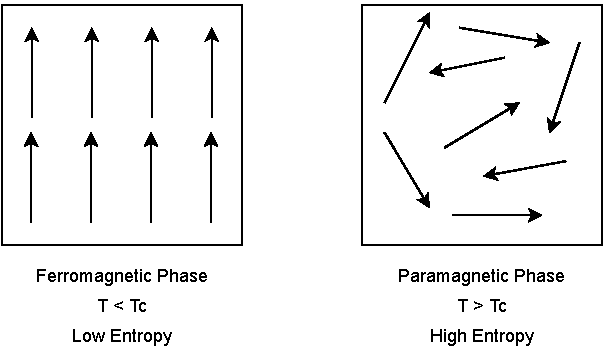
\includegraphics[scale=0.5]{spins_diagram.pdf}
\label{spins_dia}}

\caption{(a) Magnetization curve for \ce{La_{0.67}Ca_{0.33}MnO3} as a function of temperature;(b) Spins diagram for the ferromagnetic phase (left) and for the paramagnetic phase (right).}

\end{figure}

A ferromagnetic material exhibits spontaneous magnetization in the absence of an applied external magnetic field. This way, the magnetic moments of the atoms that compose the material are all naturally aligned along one direction \cite{magnetism_book}. One of the key features of ferromagnetic materials is that they only display this property below a certain well-defined critical temperature, $T_C$, usually called the Curie temperature. This temperature defines a phase transition between a ferromagnetic and a paramagnetic state, Figure \ref{tese_JA_fig1}. 
Above the Curie temperature, the entropy within the material becomes too strong and the magnetic moments start to dis-align, thus the materials looses its spontaneous magnetization, Figure \ref{spins_dia}.  In other words, the effect due to thermal disorder overtakes the ferromagnetic order.

This kind of nature is common to various transition metal, Iron, Cobalt, Nickel, and so forth, and to some rare earth materials, such as Gadolinium.
One application of ferromagnets is magnetic refrigeration. This is based on the magnetocaloric effect (MCE), which consists of a change in temperature of a magnetic material by the application and removal of an external magnetic field., known as the magnetocaloric effect (MCE). For a ferromagnetic material, the MCE is more prominent when the magnetic filed is applied for temperatures around the Curie temperature. 
High performance magnetic refrigerants include the \ce{LaFeSi} 1:13 family \cite{Fujita} and \ce{MnFeP} based intermetallics \cite{Bruck}. 

In the recent years, computational materials design is becoming the new norm to discover new materials by combining computer science with quantum and statistical mechanics. It is more advantageous than the experimental sciences since it is not as time-consuming and bounded by high costs in equipment as running an experiment \cite{Curtarolo2013,Chen2019, Sanvito2017}. 

\section{Ising Model}

In 1920 Wilhelm Lenz, a German physicist, gave Ernest Ising, his PhD student, an exercise that considered a one-dimensional chain of spin-1/2 particles that can be either pointing up or down. The spins can only interact with their neighbours. Later in 1925, Ising solved this problem, awarding him a doctorate in physics,  and concluded that there was no phase transition in the one-dimensional case and wrongly extrapolated that there was no phase transition in higher dimensions \cite{Ising1925}. It was not until 1944 that a Norwegian-born American physicist, Lars Onsager, solved the much harder two-dimensional case analytically, in a square lattice \cite{Onsager1944}. In this case, Onsager showed that there is a well defined phase transition from a ferromagnetic to a paramagnetic state at a critical temperature ($T_C$), therefore proving Ising's extrapolation wrong.

Since then, the Ising Model has become one of the most studied and published physical models, since it has a non-trivial phase transition while being able to have an analytical solution, at least for dimensions lower or equal to two. As of yet, there are no exact solutions for higher dimensions.We are only able to get properties from three dimensional lattices by numerical simulation.

The Ising Hamiltonian describes a system of lattice of atomic spins which can have two spin directions, up $(+1)$ and down $(-1)$ with neighbour to neighbour interactions. So, it is written as
\begin{equation}
	\mathcal{H} = -\sum_{<i,j>} J_{ij} S_i S_j - H \sum_iS_i
\end{equation}
where $J$ is the interaction for constant between two neighbouring particles, $S_i$ is the spin value of the particle at the site $i$, $<i,j>$ denotes that the sum is conducted over all neighbouring particles. The second term represents the interaction with an external magnetic field, $H$, and it is completely optional. If $J>0$, the system will have a ferromagnetic behaviour since parallel spins are energetically more favourable, and if $J<0$, the system will behave in an anti-ferromagnetic way.

In this work, I will not evaluate the Ising Model with an applied magnetic field, $H=0$, and consider $J_{ij}=1$ to simplify the computations. With this being said, the Hamiltonian treated in this work goes as follows,
\begin{equation}
	\mathcal{H} = -\sum_{<i,j>} S_i  S_j \equiv -\frac{1}{2} \sum_{ij} S_i S_j
\end{equation}

To simulate real materials we can obtain the values of the interaction constant for each atom in our lattice through Density Functional Theory (DFT) calculations \cite{DFT_book, Marzari2021}.

\subsection{Joint Density of States}

It is mentioned in any undergraduate course in statistical mechanics that the density of states (DoS), $g(E)dE$, gives the number of states that have a certain energy between $E$ and $E+dE$ \cite{stat_mech}. For discrete systems, like the Ising Model, the DoS evaluated at a certain energy gives us the exact number of microstates that have a specific energy $E$. Through the DoS we can obtain the partition function $Z(T)$, as a function of temperature, and then compute energy related thermodynamic variables, such as the mean energy $E(T)$, specific heat $C(T)$, Helmholtz free energy, $F(T)$.  
As we are dealing with magnetic systems our natural interest is to study the magnetization throughout various temperatures and applied magnetic field intensity. For this, we need the number of microstates with a certain pair $(E,M)$. This is the exact description of the Joint Density of States (JDoS), a multi-variable histogram with information about the number of microstates with a certain energy and another parameter, like density, $\rho$, number of particles, $N$, or, in this case, magnetization, $M$. This way we can compute the partition function as a function of both temperature and magnetization, $Z(T,M)$ and the Helmholtz free energy as $F(T,M)$.

Table \ref{exact_L2} represents the JDoS for the Ising Model in a simple square (SS) lattice with length $2$ and periodic boundary conditions (PBC). The extreme magnetization configurations appear only once in the JDoS, no matter the size of the lattice, since they represent all up or all down spins configurations. 

\begin{table}[h]
\centering
\caption{Joint Density of States for the SS lattice with $L=2$ Ising Model. The rows are the values of energy, $E$, and the columns the values of magnetization, $M$.}
\label{exact_L2}
\begin{tabular}{l|lllll}
$E \ / \ M$ & $-4$ & $-2$ &  $0$ & $+2$ &  $+4$ \\ \hline
$-8$  & 1  & 0  & 0 & 0 & 1 \\
$-4$  & 0  & 0  & 0 & 0 & 0 \\
$0$   & 0  & 4  & 4 & 4 & 0 \\
$+4$   & 0  & 0  & 0 & 0 & 0 \\
$+8$   & 0  & 0  & 2 & 0 & 0
\end{tabular}
\end{table}

\begin{figure}[h]
	\centering
	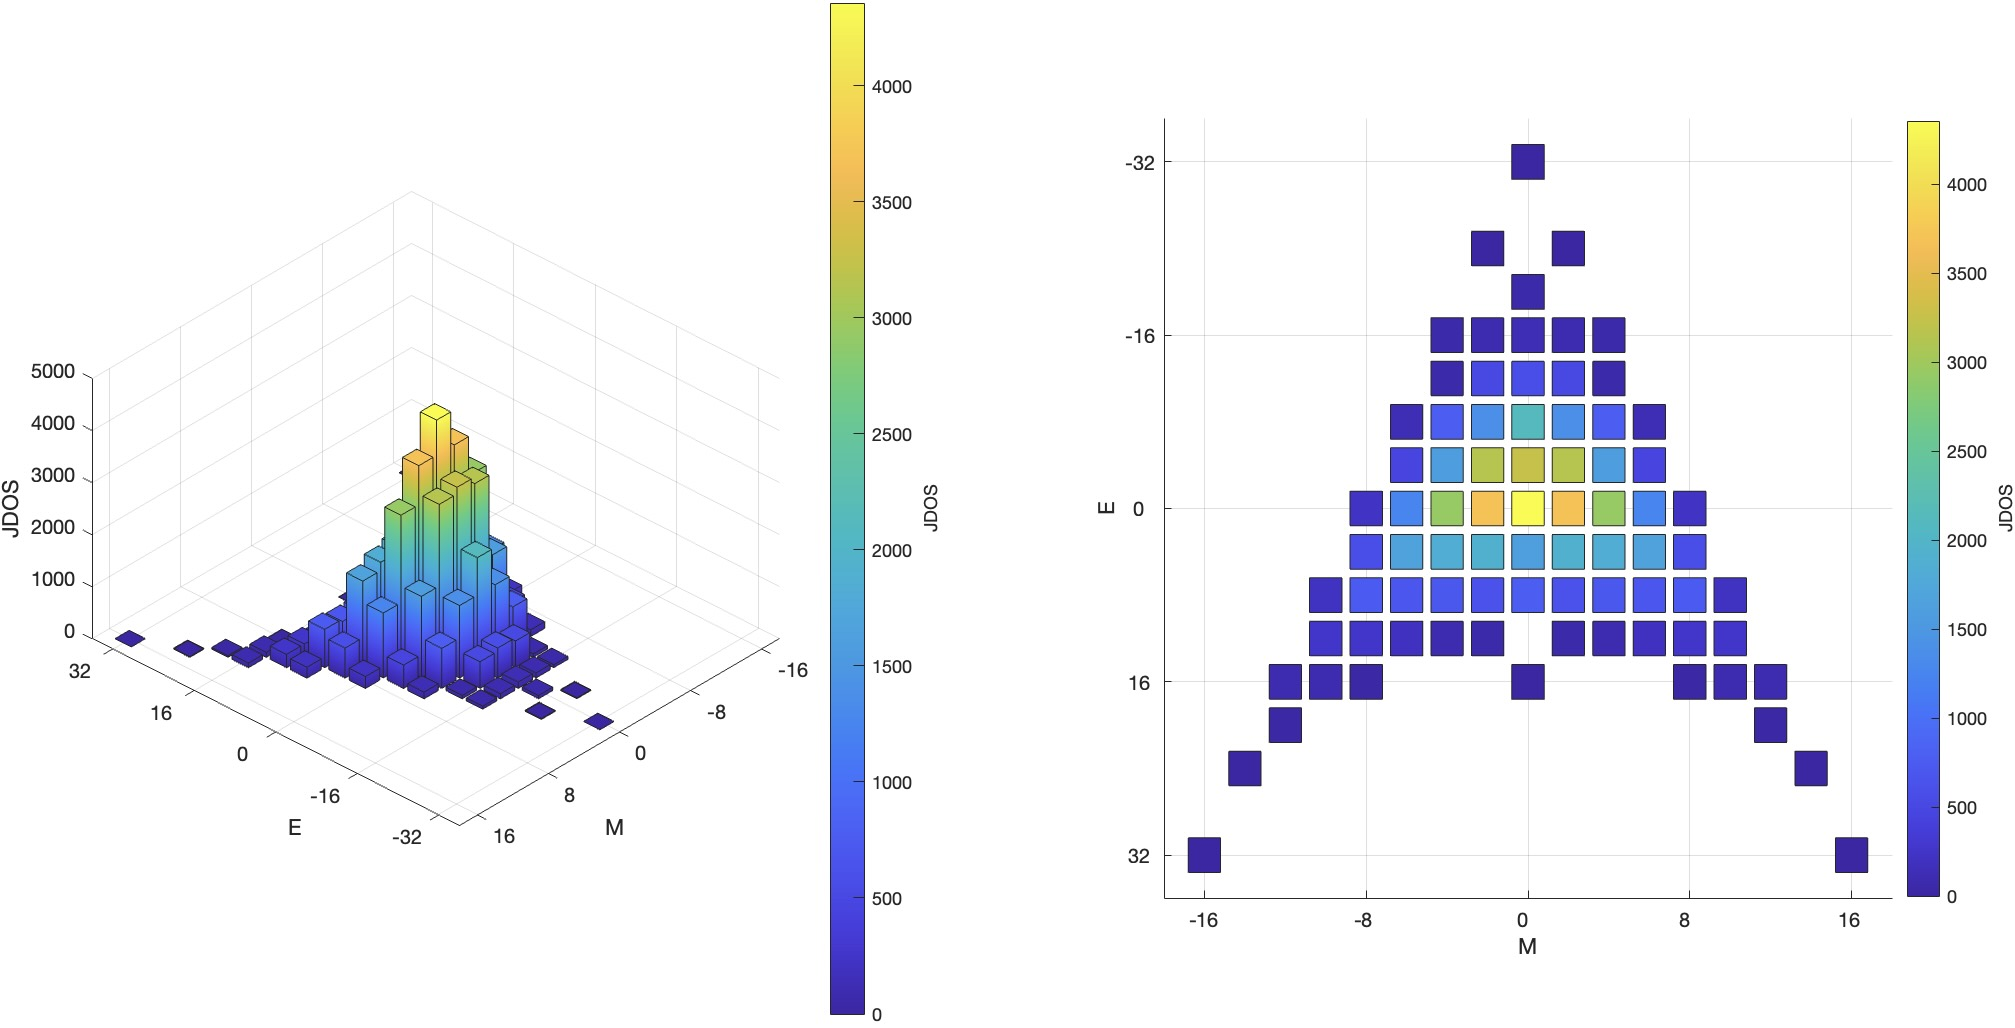
\includegraphics[scale=0.2, height=5cm]{JDOS_exact_L4_SS.jpeg}
	\caption{Plot of the exact JDoS for the SS L4 Ising Model with PBC. This was obtained by visiting each microstate available to the system.}
	\label{exact_L4}
\end{figure}

\pagebreak

There are three configurations worth noting.The first is the zero energy and zero magnetization state. This is the state with the most micro configurations since it represents the macrostate in which is likely to find the system in, when $T\gg T_C$(has the highest entropy). The second is the macrostate with the highest energy and zero magnetization. For every system size and lattice this macrostate has always $2$ microstates, since the spins are sorted in a chess/checker board pattern. The last configuration is the state with the least energy and zero magnetization. Its value is always going to be equal to $2L$, since the spins are sorted in rows and columns of alternating positive and negative spins, similar to slices. Throughout this work these configurations will appear again and they will be referred as, Zero Zero, Checker Board and Slice, respectively. 

The simplest way to compute the JDoS is to visit all of the possible microstates. It is easy to do this when we have $16$ spins ($L=4$ in a SS lattice, Figure \ref{exact_L4}), since the number of possible configurations is still quite small, $2^{16} \approx 65E3$ configurations. But, for instance, for systems with $256$ spins ($L=8$ in a SS lattice) it becomes computationally impossible to randomly or sequentially visit all of the microstates since we have to sample $2^{256} \approx	 1E77$ configurations. 
Instead we can use various clever numerical methods methods to get an estimation of the JDoS in a much more reasonable time with fairly good precision. I will present widely studied methods in the next Chapter and a new unpublished method in the third Chapter.

\subsection{Thermodynamics}

From the JDoS we can obtain all of the thermodynamic quantities when the system is in an equilibrium state. In this section I will present some useful formulas to compute those variables from the JDoS. 
The probability of a given state with energy $E_i$, is given by
\begin{equation}
	P_i = \frac{\sum_q g(E_i, M_q) \exp(-\beta E_i)}{Z},
\end{equation}
where $\beta$ is defined as $\beta \equiv 1/k_BT$ and $Z$ is the canonical partition function given by
\begin{equation}
	Z = \sum_q Z(T, M_q) = \sum_q \sum_i g(E_i, M_q) \exp(-\beta E_i).
\end{equation}
From this we can obtain mean thermodynamic variables, 
\begin{equation}
	\langle E \rangle = \frac{1}{Z} \sum_i \sum_q  g(E_i, M_q) E_i \exp(-\beta E_i),
\end{equation}
\begin{equation}
	\langle M \rangle  = \frac{1}{Z} \sum_q \sum_i M_q g(E_i, M_q) \exp(-\beta E_i) \equiv \frac{1}{Z} \sum_q M_q Z(T, M_q).
\end{equation}
$\langle E \rangle$ is related to the specific heat by 
\begin{equation}
	\langle C \rangle = \frac{\langle E^2 \rangle - \langle E \rangle^2}{\left( k_BT \right)^2},
\end{equation}
and finally to obtain the mean entropy we use the second law of thermodynamics,
\begin{equation}
	\langle S \rangle= \int \frac{\langle C \rangle}{T} dT.
\end{equation}

\pagebreak

However there is another way to estimate thermodynamic properties, from the computed JDoS.  Using the Helmholtz free energy, defined as 
\begin{equation}
	F(T, M) = - k_B ln(Z(T, M)) \equiv U - TS
\end{equation}
and the principle of minimum energy, we can extract $F_{min} (T) = \min(F(M, T))$, which is defined as the lowest temperature-dependent free energy that can be reached by the system.
From it we can obtain the magnetization and energy for that value of free energy minima, $M_{F_{min}}$ and $E_{F_{min}}$, respectively.Through $F_{min}$ we can use the following thermodynamic relations to compute the specific heat and entropy of the system:
\begin{equation}
	C = - T \frac{\partial^2 F_{min}}{\partial T^2},
\end{equation}

\begin{equation}
	S = - \frac{\partial F_{min}}{\partial T}.
\end{equation}

\subsection{Relevance}

Despite its simplicity and age, the Ising Model is used in a multitude of research fields within the physical sciences and the social sciences. 

Within the physical sciences the Ising Model is used to simulate not only magnetic materials but also systems that are characterized by nearest-neighbour interactions and undergo a phase transition Ising-like, this means systems that go from an ordered-low entropy phase to a disordered-high entropy phase at a specific critical temperature \cite{Pelissetto2002}. 
Liquid vapour transitions, where the order parameter is the density, $\rho$, binary liquid mixtures, where the order parameter is the concentration and the transition corresponds to the mixing of the two liquids.

In the social sciences, the Ising Model has been used to describe a plethora of theoretical models of social behaviour and model financial markets \cite{review_social_ising}. 
Topics ranging from the study of racial segregation in certain communities \cite{segregation}, to a demonstration that a community that speaks only one language can start speaking another one without any outside bias \cite{language_ising}.

In economics Monte Carlo methods are widely used to model financial markets due to its randomness, and the Ising Model is the standard model that those methods are applied to. In theses case studies the spins are the option of buying or selling a certain stock through neighbour to neighbour communication or external factors. The magnetization represents the average actions of the stock market agents \cite{stock_ising, eco_thesis}.












